\documentclass[11pt]{report}
\usepackage[utf8]{inputenc}
\usepackage{graphicx}
\usepackage[margin=1in]{geometry}
\usepackage{placeins}
\usepackage{glossaries}
\graphicspath{ {images/} }

\title{
{ Procedural Plant Generation and Simulated Plant Growth }\\
{\large Massey University}
\\
\vspace{2cm}
{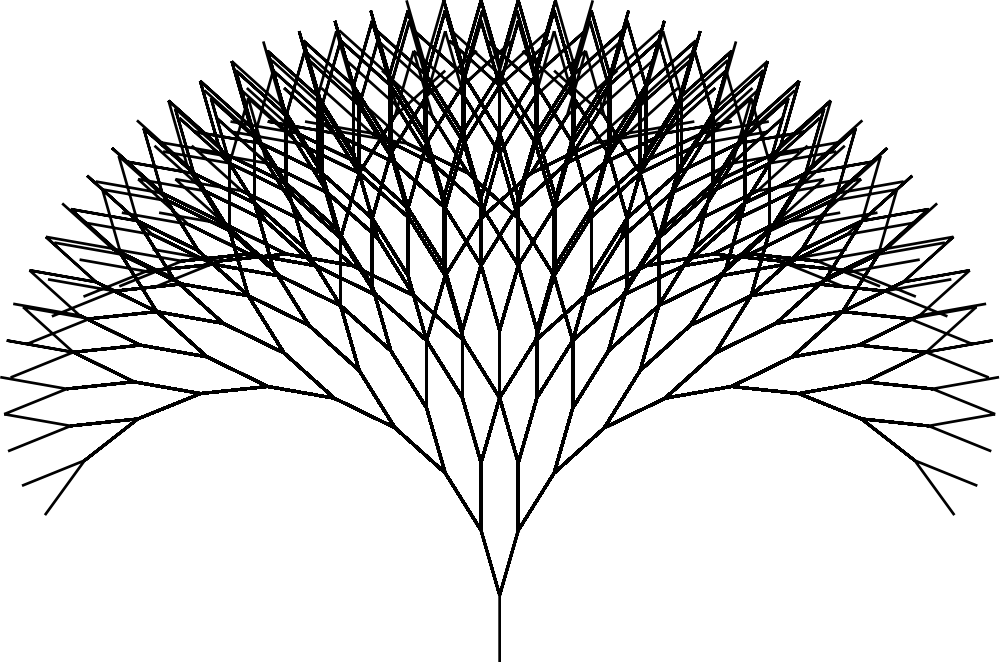
\includegraphics[scale=0.35]{titlepage.png}}
\vspace{2cm}
}


\author{Matthew Crankshaw}
\date{25 February 2019}


\makeglossaries
\newglossaryentry{C/C++}
{
	name=C/C++, 
	description={Refers to the C and C++ programming languages}
}

\newglossaryentry{OpenGL}
{
	name=OpenGL, 
	description={The Open Graphics Library is a cross-platform, cross-language application programming interface used in creating graphics applications}
}

\newglossaryentry{Lexer}
{
	name=lexer, 
	description={A computer program that performs lexical analysis}
}

\newglossaryentry{Parser}
{
	name=parser,
	description={A computer program that performs parsing}
}

\newglossaryentry{Morphology}
{
	name=morphology, 
	description={The study of the forms of things}
}

\newglossaryentry{Shader}
{
	name= shader, 
	description={A set of instructions that run on the graphics processing unit which calculates rendering effects}
}

\newacronym{2d}{2D}{Two Dimensional}
\newacronym{3d}{3D}{Three Dimensional}
\newacronym{api}{API}{Application Programming Interface}
\newacronym{bnf}{BNF}{Backus-Naur Form}
\newacronym{cfg}{CFG}{Context-Free Grammar}
\newacronym{cpu}{CPU}{Central Processing Unit}
\newacronym{eol}{EOL}{End of Line}
\newacronym{eof}{EOF}{End of File}
\newacronym{glm}{GLM}{OpenGL Mathematics Library}
\newacronym{glsl}{GLSL}{OpenGL Shading Language}
\newacronym{gpu}{GPU}{Graphics Processing Unit}
\newacronym{opengl}{OpenGL}{Open Graphics Library}
\newacronym{stl}{STL}{Standard Template Library}
\newacronym{glfw}{GLFW}{Graphics Library Framework} 
\newacronym{lerp}{LERP}{Linear Interpolation}
\newacronym{lifo}{LIFO}{Last In First Out}
\newacronym{flex}{Flex}{Fast Lexical Analyzer Generator}
\newacronym{vao}{VAO}{Vertex Array Object}
\newacronym{vbo}{VBO}{Vertex Buffer Object}

\begin{document}

\maketitle

\chapter*{Acknowledgements}

\chapter*{Abstract}

\tableofcontents
\listoffigures


\chapter{Introduction}

Here I will introduce the project and the thesis in general.


\lettrine[lines=3]{P}{}rocedurally generating 3D models of plant-life is a challenging task, largely due to the complex branching structures and variation between different types of plant species. Up until recently, all assets within 3D graphics applications either had to be sculpted using 3D modeling software, or scanned using photogrammetry, laser triangulation or some form of contact based 3D scanning. These methods are still used today but tend to be very time consuming and extremely costly. With the increase in computational power over the last few decades more emphasis has been placed on the use of produral generation. Which can be used to create complex structures such as terrain, architecture, sound and 3D models with far greater speed than previous techniques, and often much better realism than would be possible with artists. Plant-life stands as a challenge due to the thousands of species, each with their own unique structure and features. It is difficult to define a system that can represent them all in a way that is simple, understandable and accurate. The Lindenmayer System (L-system) stands as a solution to this problem, it was originally developed by Aristed Lindenmayer as a method of representing the development of multicellular organisms \cite{lindenmayer1968mathematical}. This has since gained popularity in the area of procedural generation and has been adapted to represent different types of structures. L-systems have been adapted to represent plant-life, such as trees, flowers, algea and grasses, whilst still being applicable to non-organic structures such as music, artificial neural networks and tiling patterns \cite{Prusinkiewicz1989}.\\
 
The L-system in its most basic form, is a formal grammar which contains a set of symbols or letters that belong to an \textit{alphabet}. The alphabet is used to create a starting string known as the \textit{axiom}, as well as a set of production rules. The production rules are applied to each symbol within the axiom string, each rule dictates whether or not the symbol can be rewritten and furthermore, what they will be rewritten with. In essence, a L-system uses the set of production rules to generate a resulting string of symbols which follow those production rules. The resulting strings' meaning can then be interpreted in a way that best fits what it is trying to represent. In this case the string can interpreted to generate a model of a plant. This thesis develops upon the L-system concepts described by Przemyslaw Prusinkiewicz and Aristid Lindenmayer to procedurally generate structures of plant-life in real-time. The L-system grammar allows the structure of a plant to be described in a human readable, formal grammar. The grammar can be used to specify variation in shape, size and branching structure within a particular species. Furthermore, this thesis will also investigate the use of a parameterised L-systems to provide physical properties using string rewriting. Which in turn will enable the animation and physical behaviour of the plant that it generates, thus making it possible to simulate external forces such as gravity and wind. \\

This chapter will describe the motivations behind this research and how it can be used to improve the procedural generation of plant-life in 3D applications. It will then introduce the concepts of procedural generation, rewriting systems and formal grammars. Briefly describing how procedural generation can be applied to the development of plant-life through the use of rewriting systems. Furthermore, this chapter will provide sufficient background as to the use of formal grammars as a means of describing complex L-system languages. Finally there will be an outline as to the structure of this thesis, and how this research will be conducted.

\section{Motivations}
 
One of the most time consuming parts for digital artists and animators is creating differing variations of the same piece of artwork. In most games and other graphics applications environment assets such as trees, plants, grass, algae and other types of plant life make up the large majority of the assets within a game, and creating a plant asset can take a skilled digital artist more than an hour of work by hand, The artist will often have to create many variations of the same asset in order to obtain enough variation that a user of that graphics application would not notice that the asset has been duplicated, if this is multiplied by the number of assets that a given artist will have to create or modify, there is an incredible number of hours that could have potentially been put to use creating much more intricate assets. In addition to this, it is also important to note that graphics assets are then stored in large data files, describing the geometry and textures and other information. If we require three very similar plants, we have to store three separate sets of data. Procedurally generating plants can avoid this wasteful data storage entirely, instead a relatively small L-system description can be stored which can be used to procedurally generate all the required geometry and other information during the execution of the program.\\

The L-system can not only procedurally generate the geometry of the plant-life but can also generate parameters physical properties of the plant inself such as the weight and flexibility of branches as well as its wind resistance and many other important information that can be used to simulate or animate the motion of the plant under various forces.  

\section{Introduction to Procedural Generation}

Procedural generation is used in many different areas and applications in computer graphics, particularly when generating naturally occuring structures such as plants or terrain. An effective procedural generator is capable of taking input in the form of a relatively simple description of what it should be generating, its job is then to computationally generate the structure in a way that is accurate to the description given. Currently there are three main methods for procedurally generating models of plant-life, these are genetic algorithms \cite{haubenwallner2017shapegenetics}, space colonisation algorithms\cite{juuso2017procedural} and L-systems. The genetic algorithm and space colonisation algorithms are similar in that they require the overall shape of the plant to be described by simple 3D shapes, the algorithm then creates a branching structure that matches these shapes. The limitation of these methods is that the 3D description is not very specific and although it can get good results for trees, it may not be able to generate a different types of plant-life, such as flowers. The L-system on the other hand relies on a mothod of string rewriting, whereby the rewriting is based on a set of production rules in order to generate a string of symbols that obay those rules. A separate system can later interpret this string to create the model. The L-system procedural generation therefore, has two separete systems within it, one of string rewriting and one of interpretation of the generated string. This makes it quite easy for the same L-system to generate very different results based upon the interpretation.\\

Plant-life can have very complex and seemingly random structures, however, with closer observation, trees of a similar species have obvious traits and features. For instance, a palm tree has long stright trunks with long compound leaves exclusively near the top, branching in all different directions. Comparatively a pine tree has a long staight trunk with many branches coming off in different directions pupendicular to the ground, from its base to the top of the trunk. These are two very different species of trees, the palm  belongs to the Arecaceae family, whereby the pine belongs to the Pinaceae family. They look different, however, they share very similar properties, such as their long straight trunks. The challenge behind the  procedural generation of plant-life, is providing a human readable grammar that describes in sufficient detail, how to generate a three dimensional model. Whilst allowing for randomness and variety within the generation process, such that variations of a particular species can be generated without repetition. The  grammar for procedural generation should also be relatively straightforward and intuitive, and must accurately represent what it is going to generate. Furthermore, the description must not be limited to only known species of trees, as some graphics applications may require something that is other-wordly.

\section{Introduction to Rewriting Systems}

Rewriting systems are the fundamental concept behind L-systems. In their most basic form, rewrite systems are a set of symbols or states, and a set of relations or production rules that dictate how to transform from one state to the other \cite{prusinkiewicz2012algorithmic}. Using these state transitions it is possible to generate complex structures by successively replacing parts of a initial simple object with more complex parts. Rewrite systems can be non-deterministic, meaning that there could be a transition which depends on a condition being met or on a neighbouring states. Using this rewriting concept any preceeding state can rely upon some conditions neccessary for transformation. If condition is true the state will be rewritten, otherwise it will remain the same, and will be checked in the next rewriting stage. A graphical representation of an object defined in rewriting rules can be seen below in figure \ref{snowflake curve} below, called the snowflake curve proposed by Von Koch \cite{koch1906methode}.

\begin{figure}[htbp]
	{\centering
		\setlength{\fboxrule}{1pt}
		\vspace{7px}
		\fbox{
			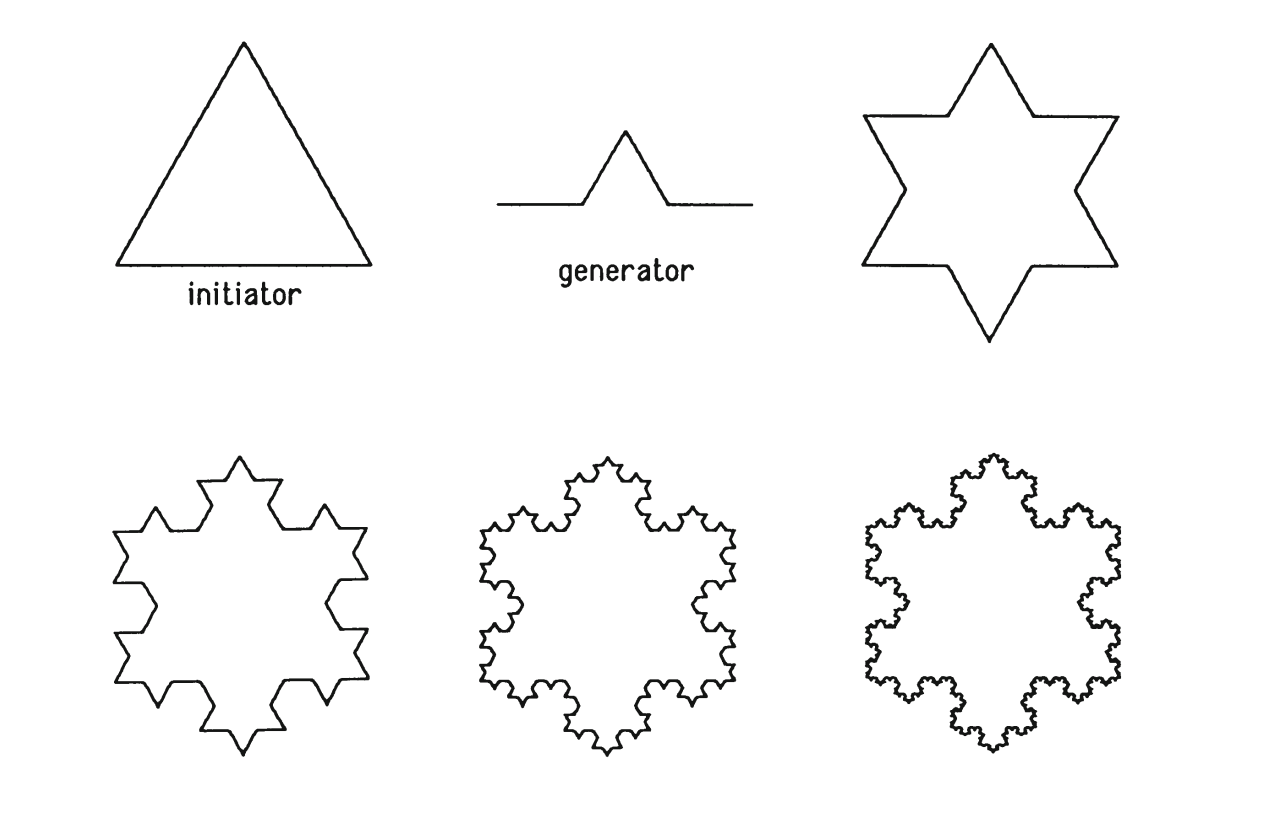
\includegraphics[scale=0.3]{Diagrams/snowflakeCurve.png}
		}
		\caption{Construction of the snowflake curve\cite{prusinkiewicz2013lindenmayer}.} \label{snowflake curve}
	}
\end{figure}
\FloatBarrier

\noindent
The snowflake curve starts with two parts, the initiator and the generator. The initiator is is the initial set of edges forming a certain shape, whereas the generator is a set of edges which can be used to replace each edge of the initiator to form a new shape. That new shape then becomes the initiator for the next generation, where each edge is again replaced by the generator. The result is a complex shape similar to that of a snowflake. The initiator, generator concept is a graphical representation of how rewriting systems operate, rather than the initiator and generator being a set of edges they are instead represented by a set of symbols or strings.

\section{Introduction to Formal Grammars}

In the context of computer science, grammars are defined as a set of rules governing which strings are valid or allowable in a language or text. They consist of syntax, morphology and semantics. Formal languages have been defined in the form of grammars to suit particular problem domains. It is natural for humans to communicate a problem or solution in the form of language, it is therefore intuitive to use a language to describe the desired outcome when dealing with the procedural generation of plant-life. In the past, formal grammars have been used extensively in computer science in the form of programming languages in which humans can provide a computer with a set of instructions to carry out in order to gain an expected result. The challenge is therefore to create a  grammar in the form of a rewriting system that facilitates the procedural generation of plant-life. A rewriting system such as the L-system operates in a way that is consistant with a context-free class of Chomsky grammar \cite{chomsky1956three}, similar to that of the programming language ALGOL-60 introduced by Backus and Naur in  1960\cite{backus1960report}. In figure \ref{chomsky grammars} below, there are two types of L-system grammars that overlap the classes of chomsky grammars, the OL-system and the 1L-system. The details of these two systems will be discussed in detail chapter \ref{l-system chapter}, but in summary, 0L-systems are grammars that can represent a context-sensitive Chomsky grammar but generally tend to be context-free, the main difference between the 0L-system and the 1L-system is that 1L-systems can be recursively enumerable. Furthermore, it is possible for a 1L-system to represent any 0L-system, therefore, 1L-system languages tend to be more complex and verbose when compared to 0L-systems, this creates a trade off between a more powerful and complex language or a less powerful but simpler language. 

\begin{figure}[htbp]
	{\centering
		\setlength{\fboxrule}{1pt}
		\vspace{7px}
		\fbox{
			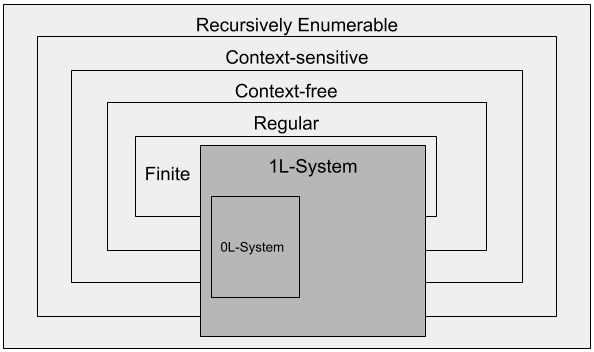
\includegraphics[scale=0.5]{Diagrams/ChomskyGrammar.png}
		}
		\caption{Diagram of the Chomsky hierarchy grammars with relation to the 0L and 1L systems generated by L-systems.} \label{chomsky grammars}
	}
\end{figure}
\FloatBarrier

\section{Structure of Thesis}

This thesis is split into three major parts. Part 1 focuses on the L-system itself, it defines the various types of L-systems for modeling plant-life, the concept of a parametric L-system as well as some techniques for definiting randomness and stochasticisity within an L-system in order to create variaty. Part 2 talks about the L-system rewriter implementation, covering how the L-system generates the resulting string and structures relavant rendering. Part 3 focuses on the interpretation and renderer implementation and how to render a convincing model of a tree on the screen, as well as simulation and animation of the generated plants.







\chapter{Outline}

\begin{flushleft}

Aristid Lindenmayer is a well known biologist who started work on what would become known as the Lindenmayer System or L-system for short. Lindenmayer initially intended the L-systems to be to be used as a way to describe the development of simple organisms such as algae and bactaria. More recently the concept has been adapted to be used to describe larger organisms such as plants and trees. L-systems have also been used to describe non organic structures like music. \cite{worth2005growing} \\

\vspace{5mm}

An L-system at its core is a formal grammar made up of an \textit{alphabet} of symbols which are put together into strings, a set of rules is used to determine whether or not a symbol in the string should be rewritten with another symbol or string. What we end up with is a string of symbols which we can refer to as a set of states, for each state the rules determine what symbols to rewrite and what they should be replaced with or if they should be replaced at all.\\

\vspace{5mm}


In section \ref{Simple DOL-systems} below, I will be going into detail about a simple type of L-system called a Deterministic 0L-system.  D0L-systems serve as a good way to introduce the concept of an L-system.

\end{flushleft}

\section{Simple DOL-system} \label{Simple DOL-systems}

\begin{flushleft}

According to Prusinkiewicz and Hanan a simple type of L-systems are those known as deterministic 0L systems, where the string refers to the sequence of cellular states and the term '0L system' abbreviates 'Lindenmayer system with zero-sided interactions'.  With D0L systems there are only three major parts. There is a set of symbols known as the (\textit{alphabet}), the starting string or (\textit{axiom}) and the state transition rules (\textit{rules}). The alphabet is a set of states. The starting string or \textit{axiom} is the starting point containing one or more states. The transition rules dictate whether a state should remain the same or transition into a different state, remain the same or even disappear. \cite{prusinkiewicz2013lindenmayer}. \\

\vspace{5mm}

Below is an example of a deterministic 0L system: \\

\vspace{5mm}

We are given the \textit{alphabet} with symbols: A, B \\ 
The \textit{axiom}: A \\
The \textit{rule} set: \\ 
A $\rightarrow$ AB \\
B $\rightarrow$ A \\

\vspace{5mm}

The symbol $\rightarrow$ can be verbalised as "replaced by". Therefore the first rule is said to be, string 'A' is replaced by string 'AB' and the second rule is said to be 'B' is replaced by the string 'A'.\\
To start we take the first state in the \textit{axiom} which, in this case is the symbol 'A', we then check it against the first rule which is 'A', if the current state matches the rule state we replace 'A' with whatever the rules successor is, which is 'AB'. We would then move onto the next state in the axiom, however there is only one state in the axiom, 'A' so we are finished with the first generation. The states 'AB' then becomes the new starting string for the first generation. We can then continue by matching the rules once again to the new starting string. Below I have shown the string for each generation up to the sixth generation.\\

\vspace{5mm}

0.) A \\
1.) AB \\
2.) ABA \\
3.) ABAAB \\
4.) ABAABABA \\
5.) ABAABABAABAAB \\

\vspace{5mm}

This rewriting of strings using a set of rules is ultimately the underlying concept behind L-systems. There are a number of improvements that can be made to this type of L-system in order to accommodate for more complex and intricate structures. I will be talking about these in more detail in the following sections, however some important imporovements are: constants, variables, branching constructs, parametric l-systems, conditional rules and random values. //

\vspace{5mm}

An example of how an L-system can represent a real life biological structure would be Prusinkiewicz and Lindenmayer's simulation of a blue-green bacteria known as \textit{Anabaena catenula}\\

\vspace{5mm}

Prusinkiewicz and Lindenmayer created the following DOL-system representation shown below in the following grammar: \\

\vspace{5mm}

$w$ : $ a\textsubscript{r} $\\
\textit{p1} : $ a\textsubscript{r} $ $\rightarrow$ $a\textsubscript{l}b\textsubscript{r}$ \\
\textit{p2} : $ a\textsubscript{l} $ $\rightarrow$ $b\textsubscript{l}a\textsubscript{r}$ \\
\textit{p3} : $ b\textsubscript{r} $ $\rightarrow$ $a\textsubscript{r}$ \\
\textit{p4} : $ b\textsubscript{l} $ $\rightarrow$ $a\textsubscript{l}$ \\

\vspace{5mm}

The value $w$ is there to specify the axiom which is this case has the value of $ a\textsubscript{r} $. \textit{p1}, \textit{p2}, \textit{p3}, \textit{p4} are the names of the rules that follow after the semi-colon. In order to simulate Anabaena catenula we need four rules. \\
According to Prusinkiewicz and Lindenmayer "Under a microscope, the filaments appear as a sequence of cylinders of various lengths, with $a$-type cells longer than $b$-type cells. And the subscript $l$ and $r$ indicate cell polarity, specifying the positions in which daughter cells of type $a$ and $b$ will be produced. \cite{prusinkiewicz2012algorithmic} \\

\vspace{5mm}

The first five generations can be written as follows: \\

\vspace{5mm}

0.) $a_r$ \\
1.) $a_l b_r$ \\
2.) $b_l a_r a_r$ \\
3.) $a_l a_l b_r a_l b_r$ \\
4.) $b_l a_r b_l a_r a_r b_l a_r a_r$ \\
5.) $a_l a_l b_r a_l a_l b_r a_l b_r a_l a_l b_r a_l b_r$ \\

\vspace{5mm}



\end{flushleft}

\section{Constants and Variables}

\begin{flushleft}

Constants are symbols or states which don't have any significant value during the rewriting process and therefore will remain the same between generations however they do have significance when the final string is being interpreted and furthermore represented. There are a number of constants that have a fixed meaning when interpreted and are therefore known as commands. These values are:

\vspace{5mm}

$\bullet$ F: 				\hspace{10mm}  		Move forward by a specified distance whilst drawing a line \\
$\bullet$ f: 				\hspace{10mm} 		Move forward by a specified distance without drawing a line \\
$\bullet$ +: 				\hspace{10mm} 		Yaw to the right specified angle. \\
$\bullet$ -: 				\hspace{10mm} 		Yaw to the left by a specified angle.  \\
$\bullet$ /: 				\hspace{10mm} 		Pitch up by specified angle. \\
$\bullet$ $\backslash$: 	\hspace{10mm} 		Pitch down by a specified angle.  \\
$\bullet$ $\hat{}$: 		\hspace{10mm} 		Roll to the right specified angle. \\
$\bullet$ \&:				\hspace{10mm}  		Roll to the left by a specified angle.  \\

\vspace{5mm}

The question then remains why should they be interpreted using these commands and how are these instructions actually interpreted. As with any grammar, there is a number of ways of interpreting the string that is generated. One method proposed by Przemyslaw Prusinkiewics is "to generate a string of symbols using an L-system, and to interpret this string as a sequence of commands which control a 'turtle'" \cite{prusinkiewicz1986graphical}.\\

\vspace{5mm}

When talking about a turtle, prusinkiewicz is refering to turtle graphics. Turtle graphics is a type of vector graphics that can be carried out with instructions. It is named a turtle after one of the main features of the Logo programming language. The simple set of turtle instructions shown below, can be expressed in the form below and displayed as figure \ref{basic turtle}\\

\vspace{5mm}

1. Move forward by 1.\\
2. Rotate right by 90 degrees.\\
3. Move forward by 1.\\
4. Rotate left by 90 degrees \\
5. Move forward by 1. \\
6. Rotate left by 90 degrees. \\
7. Move forward by 1. \\
8. Rotate right by 90 degrees. \\
9. Move forward by 1.\\

\vspace{5mm}

\begin{figure}[htbp]
	{\centering
		\vspace{7px}
		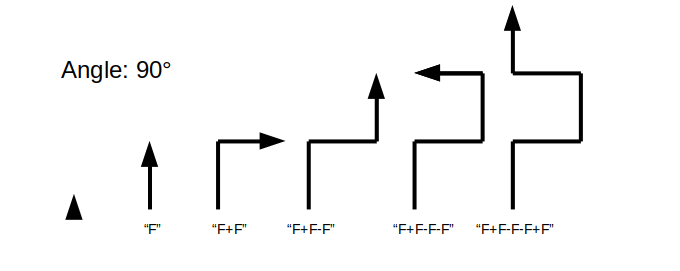
\includegraphics[scale=0.5]{Diagrams/basic_turtle.png}
		\caption{Diagram showing a turtle interpreting simple L-system string.} \label{basic turtle}
	}
\end{figure}
\FloatBarrier

\vspace{5mm}

There are a further two commands which I will be covering in detail in section \ref{branching}. We can also have constant numerical values that can be used. For instance we could pass in a constant value of 1.0 as a parameter to the forward instruction as follows.

\vspace{5mm}

F(1.0)+F(1.0)-F(1.0)+F(1.0)

\vspace{5mm}

In doing this, we are able to specify that we would like to move forward by a specified amount. In this case we would like to move forward by 1.0 unit length. We will be covering parametric L-systems in great detail in section \ref{parametric}.

\end{flushleft}

\section{Branching} \label{branching}

\begin{flushleft}

In the previous section there are two turtle commands in particular which were  not covered. These are the square bracket commands "[", "]". The square bracket characters instruct the turtle object to save its position and rotation for the purpose of being able to restore that saved position and rotation later on. This allows the turtle to jump back to a previous position, facing the same direction as it was before. We can then branch off in a different direction.\\

\vspace{5mm}

A way to keep track of these saved locations, is in the form of a stack structure. Each time the "[" is called the current position and orientation of the turtle is saved to the top of the stack. While conversely when the "]" is called we restore the turtles position back to whatever position and orientation is stored on the top of the stack. \\

\vspace{5mm}

An example of this can be shown below in figure 2.2.\\

\begin{figure}[htbp]
	{\centering
		\vspace{7px}
		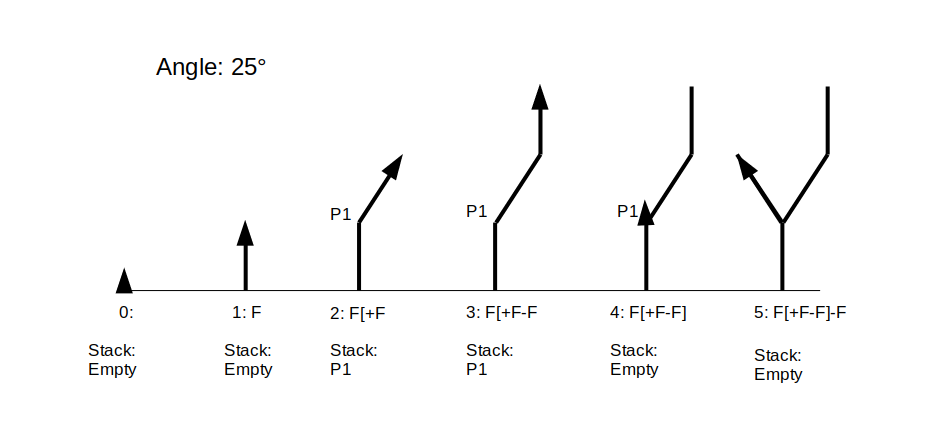
\includegraphics[scale=0.5]{Diagrams/branching_turtle.png}
		\caption{Diagram showing a turtle interpreting an L-system incorporating branching.}
	}
\end{figure}
\FloatBarrier

\end{flushleft}

\section{Parametric L-system} \label{parametric}

With simplistic L-systems like the algae representation above, there are a number of details that are skipped over when making this simplistic representation. (talk about the representation for both parameterized and non parameterised Algae systems). When it comes to representing trees as L-systems a simplistic approach would be to just assume that the width and length of each branch section is constant and will not vary depending on where in the tree it is. We can also assume that the angles at which a branch may split is also constant, say 25 degrees. 
The resulting representation of this L-system is a tree like structure, however it is not a very accurate representation of a real tree in nature. \\
In order to more accurately model trees we need to take into account the branch width, height, branching angles. There are two different approaches to solving this added complexity. One would be to increase the complexity of the L-system grammar and the other would be to increase the complexity of the interpretation of the L-system. \\
For instance defining an complex L-system grammar with a less complex interpreting system can give a huge amount of flexibility to define parameters that can accurately define exactly how the L-system should be interpreted, and because the complexity is with the L-system rewriting you also have the control of being able to change the L-system rules. \\
\\ 
A parametric l-system be represented as the following: \\
\\
\hspace*{3cm} n = 8\\
\\
\hspace*{3cm} R 1.456\\
\hspace*{3cm} r1 85\\
\hspace*{3cm} wr 0.707\\
\\
\hspace*{3cm} w : A(5)\\
\\
\hspace*{3cm} p1 : A(w) : * : F(1)!(w)[/(r1)A(w*wr)][$\backslash$(r1)A(w*wr)]\\
\hspace*{3cm} p2 : F(s) : * : F(s*R)\\
\\
The above l-system gives the resulting representation shown below in figure 3.8. 

\begin{figure}[htbp]
	{\centering
		\vspace{7px}
		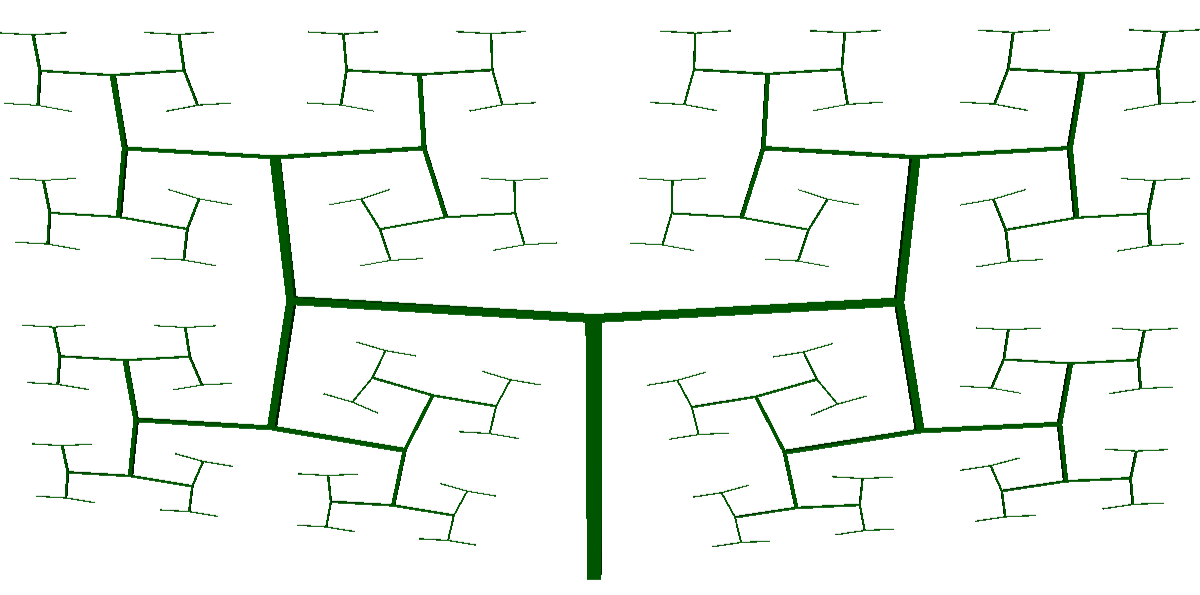
\includegraphics[scale=0.20]{ParametricLsystem/branchingPattern.png}
		\caption{3D Parametric L-system.}
	}
\end{figure}

Similarly to the 2D L-system in section \ref{Simple DOL-systems}, n refers to the number of iterations that we would like to rewrite the L-system. w refers to the Axiom string, the \#define R 1.456 states that there is a constant number that will be used somewhere in the production rules, with the name R and the value 1.456. P1, P2 refer to the production rules. The 3D L-system introduces the concept of a module.\\
A module is an instruction or variable which has zero or more parameters. The Axiom A(5) is a module with one parameter which is the number 5. A parameter can either be a number, variable or even an expression of variables and numbers. For instance A(a + 1, a * b) is a valid module A with two parameters a + 1 and a * b, where a and b are variables, however this is only a valid module if the value of a and b can be determined. Each module is treated as a single instruction, it will either be overwritten when matched with a production rule or the expression of each parameter is evaluated and is left unchaged for use when interpretted.\\
Each production rule is made up of four parts the name, the predecessor module, the condition and the successor modules, each part is separated by a colon. Therefor the predecessor for p1 is A(w), the condition is a '*' which means that in this case there are no conditions, and the successor is F(1)!(w)[/(r1)A(w*wr)][$\backslash$(r1)A(w*wr)]\\
\\
Initially we iterate through the Axiom modules and compare them to the production rule. A match is determined if they meet three criteria.\\
\\
$\bullet$ The name of the axiom module matches the name of the production predecessor. \\
$\bullet$ The number of parameters for the axiom module is the same as the number of parameters for the production predecessor. \\
$\bullet$ The condition of the production evaluates to true. If there is no condition then the result is true by default.\\
\\










\chapter{Introducing Lindenmayer Systems}

Aristid Lindenmayer is well known biologist who started work on what would become known as the Lindenmayer System or L-system for short. Originally L-systems were intended to be used as a grammar for describing the development of simple organisms. However over the years they have been found to be useful in describing larger organisms and even non organic structures like music. \cite{worth2005growing} \\
\\
In order to talk about the more complex L-systems such as the 2L-system which is used to describe structures like plants and trees. I first need to talk about how L-systems are described as well as how string rewriting works. The most simple form of L-system is a non parametric DOL-system.    

\section{The Use of L-systems in 3D applications}

L-systems have been talked about and researched since its inception in 1968 by Aristid Lindenmayer. Over the years it's usefulness in modelling different types of plant life has been very clear, however its presence has been quite absent from any mainstream game engines for the most part, these engines relying either on digital artists skill to develop individual plants or on 3rd party software such as SpeedTree. These types of software use a multitude of different techniques however their methods are heavily rooted in Lindenmayer Systems. 

\section{L-system grammars}

According to Prusinkiewicz and Hanan a simple type of L-systems are those known as deterministic 0L systems, where the string refers to the sequence of cellular states and '0L system' abbreviating 'Lindenmayer system with zero-sided interactions'.  With 0L systems there are only three major parts. There is a set of symbols (\textit{alphabet}), the starting string (\textit{Axiom}) and state transition rules (\textit{rules}). The alphabet is a set of states. The starting string is a starting point containing one or more states. The transition rules are rules that dictate whether a state should remain the same or transition into a different state or even disappear. \cite{prusinkiewicz2013lindenmayer}. \\
\\
An example of a deterministic 0L system is that a simplified model for the growth of algae: \\
\\
We are given the \textit{alphabet}: A, B \\ 
and the \textit{axiom}: A \\
and the \textit{rule} set: \\ 
A $\rightarrow$ AB \\
B $\rightarrow$ A \\
\\
If we then apply the rules to the L-system we find it creates the following generation structure. \\
1.) A \\
2.) AB \\
3.) ABA \\
4.) ABAAB \\
5.) ABAABABA \\
6.) ABAABABAABAAB \\
\\
This rewriting of initial string using a set of rules is ultimately the underlying concept behind L-systems. There are a number of improvements that can be made to this type of L-system in order to accommodate for more complex and intricate structure. One of which is the inclusion of \textit{constants}. Constants can be considered any state that does not have a rule associated with it or remains the same from generation to generation and therefore holds a consistent value or meaning. Some examples of constants are stated below. \\
\\
$\bullet$ +: Rotate to the right specified angle. \\
$\bullet$ -: Rotate to the left by a specified angle.  \\
$\bullet$ [: Save the current position and angle. \\
$\bullet$ ]: Load a saved position and angle. \\
\\
These types of constants are useful when we are dealing with fractal structures.

\section{Basic 2D L-systems} 

There are a number of fractal geometry that have become well known particularly with regards to how they can seemingly imitate nature \cite{mandelbrot1982fractal}. Particularly with the geometry such as the Koch snowflake which can be represented using the following L-system.

\begin{figure}[htbp]
	\raggedright
	\textbf{\underline{Koch Curve:}} \\
	\textbf{Alphabet:} F \\
	\textbf{Constants:} +, - \\
	\textbf{Axiom:} F \\
	\textbf{Angle:} 90$^\circ$ \\
	\textbf{Rules:} \\
	F $\rightarrow$ F+F--F+F\\
	{\centering
		\vspace{7px}
		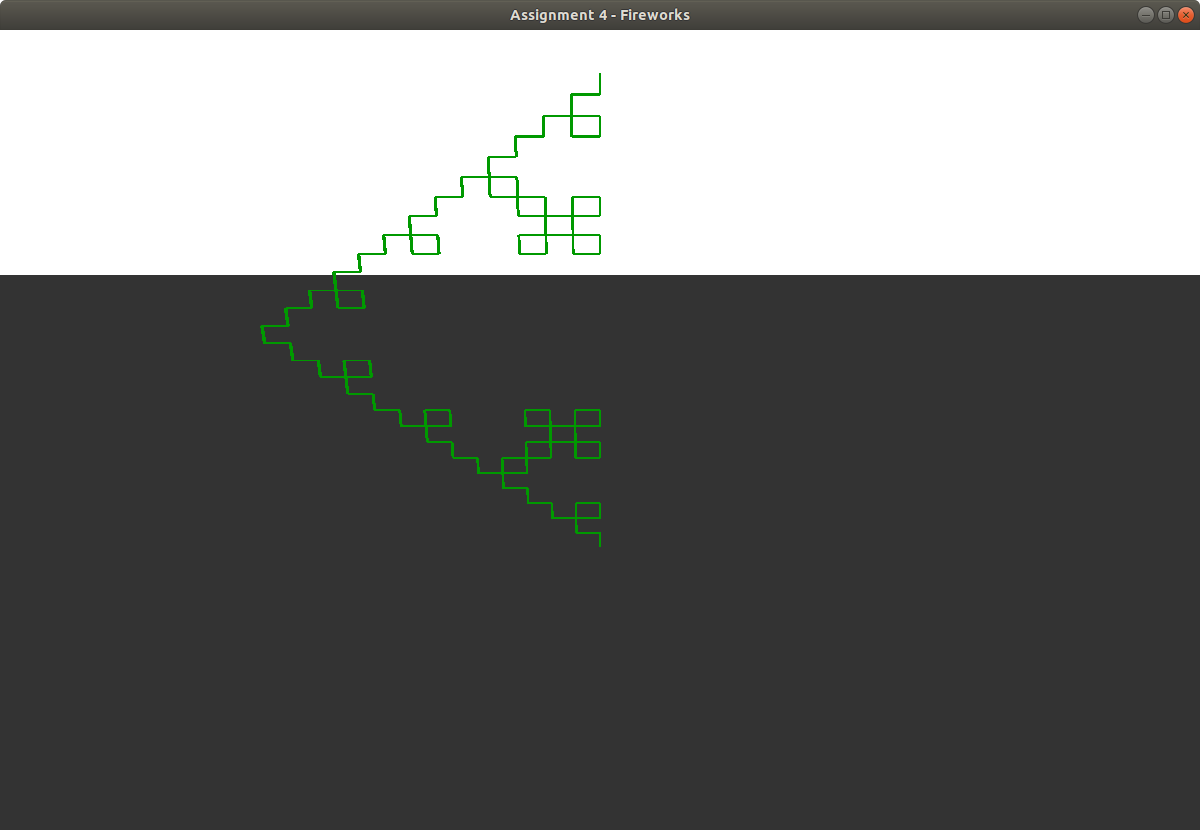
\includegraphics[scale=0.8]{KochCurve/KochCurve04.png}
		\caption{Koch Curve.}
	}
\end{figure}
\begin{figure}[htbp]
	\raggedright
	\textbf{\underline{Sierpinski Triangle:}} \\
	\textbf{Alphabet:} A, B \\
	\textbf{Constants:} +, - \\
	\textbf{Axiom:} A \\
	\textbf{Angle:} 60$^\circ$ \\
	\textbf{Rules:} \\
	A $\rightarrow$  B-A-B \\
	B $\rightarrow$ A+B+A\\
	{\centering
		\vspace{7px}
		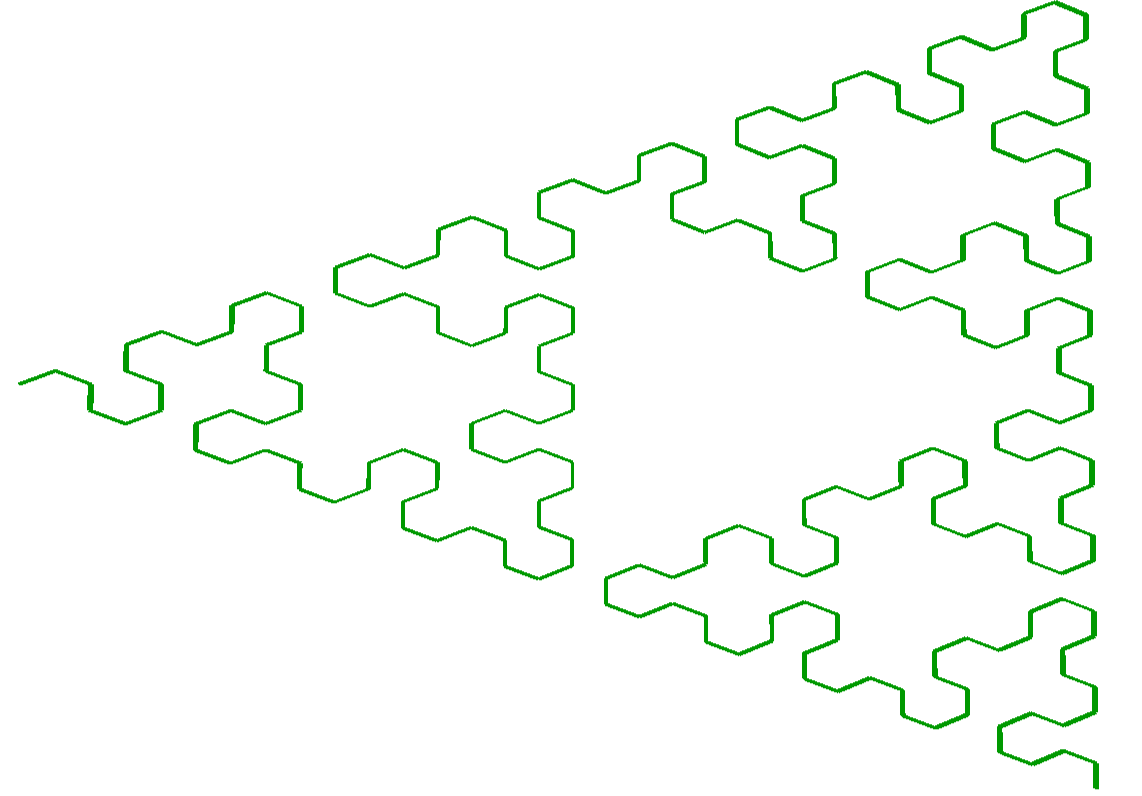
\includegraphics[scale=0.17]{SierpinskiTriangle/SierpinskiTriangle06.png}
		\caption{Sierpinski Triangle.}
	}
\end{figure}
\begin{figure}[htbp]
	\raggedright
	\textbf{\underline{Dragon Curve:}} \\
	\textbf{Alphabet:} F, X, Y \\
	\textbf{Constants:} +, - \\
	\textbf{Axiom:} FX \\
	\textbf{Angle:} 90$^\circ$ \\
	\textbf{Rules:} \\
	X $\rightarrow$ X+YF+ \\
	Y $\rightarrow$ -FX-Y\\
	{\centering
		\vspace{7px}
		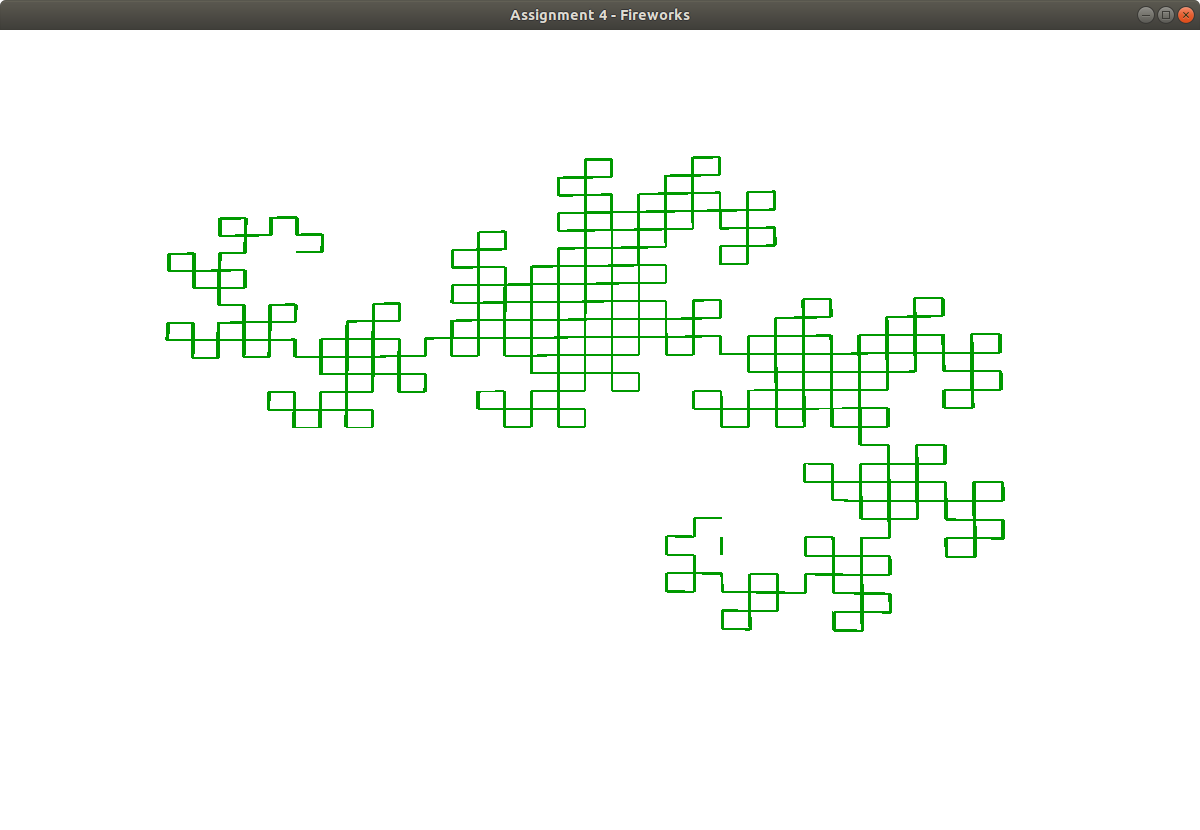
\includegraphics[scale=0.17]{DragonCurve/DragonCurve10.png}
		\caption{Dragon Curve.}
	}
\end{figure}
\begin{figure}[htbp]
	\raggedright
	\textbf{\underline{Fractal Plant:}} \\
	\textbf{Alphabet:} X, F\\
	\textbf{Constants:} +, -, [, ] \\
	\textbf{Axiom:} X \\
	\textbf{Angle:} 25$^\circ$ \\
	\textbf{Rules:} \\
	X $\rightarrow$ F-[[X]+X]+F[+FX]-X\\
	F $\rightarrow$ FF \\
	{\centering
		\vspace{7px}
		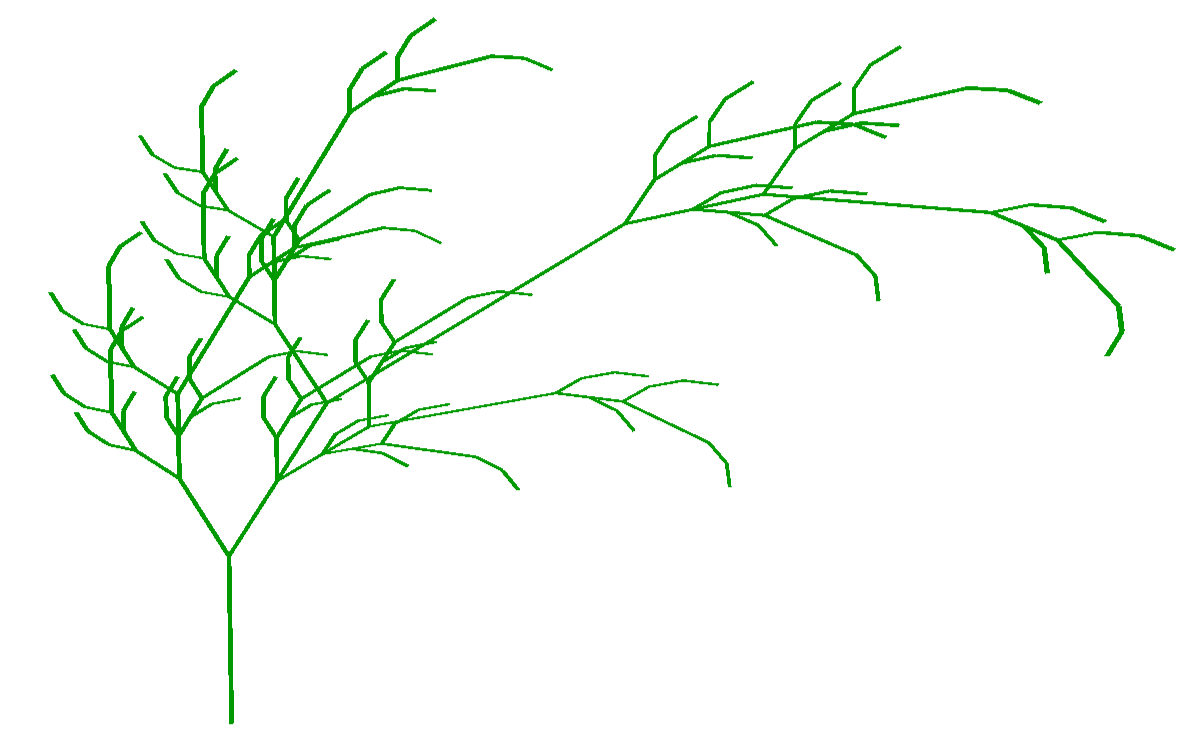
\includegraphics[scale=0.15]{FractalPlant/FractalPlant05.png}
		\caption{Fractal Plant.}
	}
\end{figure}
\begin{figure}[htbp]
	\raggedright
	\textbf{\underline{Fractal Bush:}} \\
	\textbf{Alphabet:} F\\
	\textbf{Constants:} +, -, [, ] \\
	\textbf{Axiom:} F \\
	\textbf{Angle:} 25$^\circ$ \\
	\textbf{Rules:} \\
	F $\rightarrow$ FF+[+F-F-F]-[-F+F+F]\\
	{\centering
		\vspace{7px}
		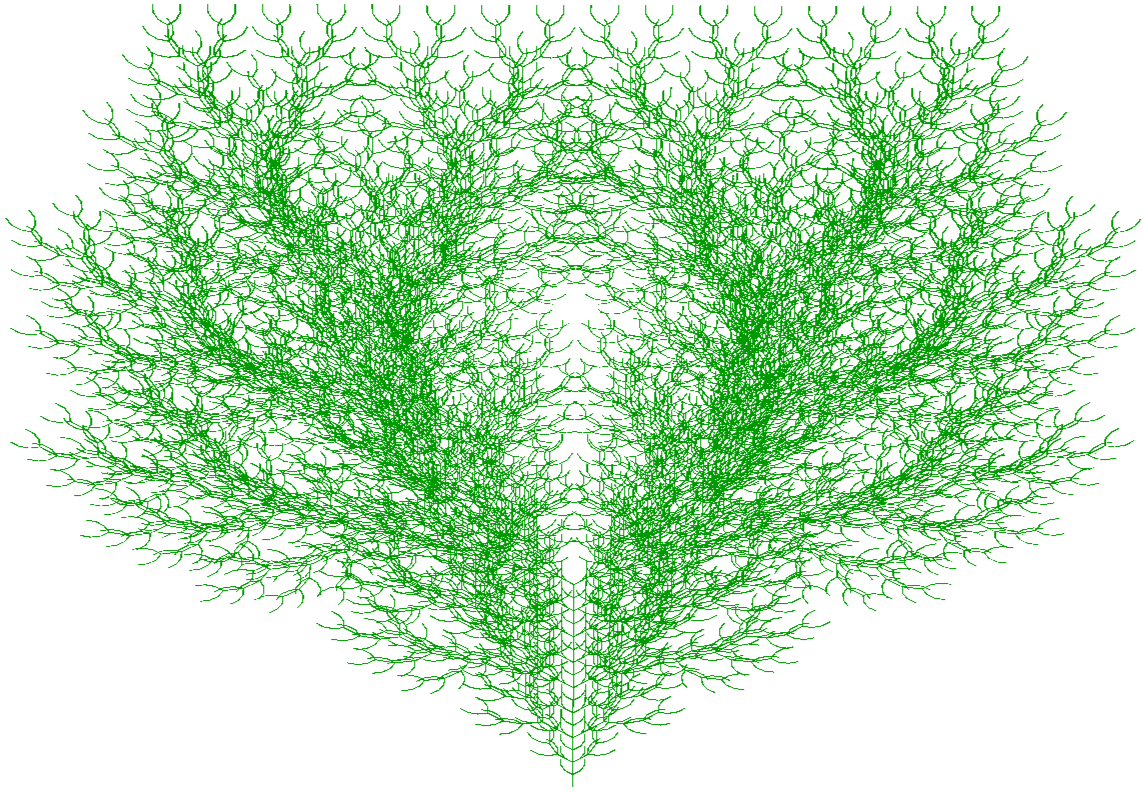
\includegraphics[scale=0.15]{FractalBush/FractalBush06.png}
		\caption{Fractal Bush.}
	}
\end{figure}

\FloatBarrier
\newpage
\section{Branching Filaments}

\chapter{Implementation}

Introduction to the implementation section

\section{Motion Equations}

Torque\\
$ \tau = I\alpha $ \\
$ \tau = f \otimes R $ \\
\\
Mass \\
$ M = \Pi~ r ^ 2 h $ 

Inertia\\
$ I = \frac{1}{3} M L ^ 2 $ \\ 
\\
Angular Acceleration\\
\\
$ \omega = \omega _0 \alpha t $ \\
\\
Next angle equation\\
$ \theta = \theta _0 + \omega _0 t + \frac{1}{2} \alpha t ^2 $ \\
\\

\section{Hook's Law}

$ f = -k _s x $\\
$ f = -k _s x + k _d v $\\

\chapter{Glossary}
\clearpage
\printglossaries

\appendix
\chapter{Appendix}
\section{Appendix 1}

\section{Bibliography}
\bibliography{chapters/ref}
\bibliographystyle{apalike}






\end{document}



